\documentclass{article}
\usepackage[utf8]{inputenc}

\title{Literature review thesis}
\author{Verheyen Willem}
\date{December 2020}

%packages
\usepackage[dutch]{babel}
\usepackage{multicol}
\usepackage[margin=0.5in]{geometry}
\usepackage{float}
\usepackage{graphicx}

%settings
\bibliographystyle{abbrv}

\begin{document}

\maketitle
\begin{multicols*}{2}

% wat, waarom, hoe, soorten, defense
\section{Introductie}

Artificiële intelligentie en machine learning worden extensief gebruikt in het hedendaagse leven, van een digitale personal assistent zoals \textit{Siri} of een recommandatie systeem die je gepersonaliseerde series aanbeveelt tot autonoom besturen van voertuigen en automatische diagnose van patiënten in een ziekenhuis. Het is belangrijk dat dergelijke kritieke applicaties betrouwbaar zijn en bestendig tegen aanvallen. \\
In deze studie behandelen we de zwakheden van machine learning modellen in de context van de intenties van de aanvaller en de verdediging die dergelijke aanvallen vermijden. 

\section{Zwakheden van machine learning modellen}
\subsection{Types van zwakheden}
In 2014-2015 toonde Szegedy et al. \cite{szegedy2014intriguing} en opvolgend werk \cite{goodfellow2015explaining} aan dat deep learning modellen vatbaar zijn voor aanvallen waarbij er een input minimaal wordt geperturbeerd en vervolgens foutief wordt geclassificeerd door het deep learning model. Deze geperturbeerde inputs die tot mis-classificatie leiden noemt men \textit{adversarial examples}.

\begin{figure}[H]
    \centering
    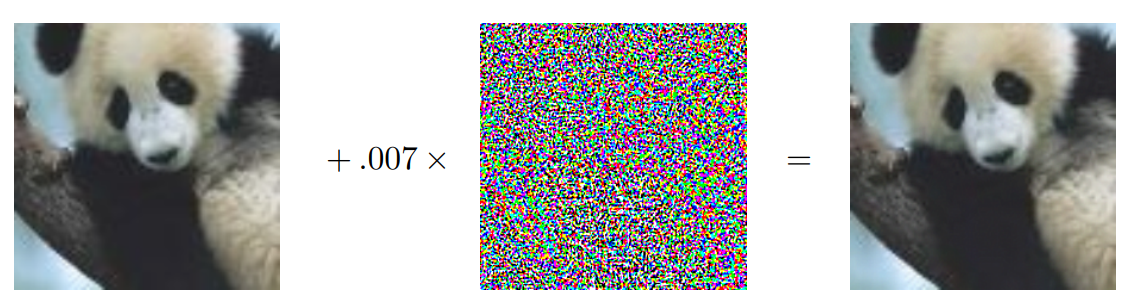
\includegraphics[width=0.4\textwidth]{panda_expl.png}
    \caption{Voorbeeld van een adversarial example toegepast of GoogleNet zoals beschreven in \cite{goodfellow2015explaining}. (links) De originele input die geclassificeerd wordt als een panda, (midden) noise die wordt toegevoegd aan de input, (rechts) de \textit{adversarial example} die foutief wordt geclassificeerd als een gibbon}
    \label{fig:adv_ex}
\end{figure}

Adversarial examples zijn een vorm van \textbf{evasion attacks} (of detection attacks) \cite{Biggio_2013} waarbij het doel is om een input te genereren die door een persoon correct geclassificeerd wordt maar niet door het machine learning model. Een andere manier om een machine learning model te exploiteren is door het gebruik te maken van \textbf{posioning attacks}, deze gebeuren in de training fase en niet in de test fase zoals het geval is evasion attacks. Bij een posioning attack worden er foutieve samples in de training data geïnjecteerd met de bedoeling om de integriteit of the toegankelijkheid van het systeem te beïnvloeden. \\
Een laatste vorm van aanvallen zijn \textbf{privacy attacks}, hierbij wordt er een machine learning model gequeryd om zo informatie op te vragen over het model en het model mogelijk te repliceren of informatie over de trainingsdata te verkrijgen. \\
In de volgende secties beschouwen we enkel evasion attacks aangezien deze relevant zijn voor het onderzoek dat we gaan verrichten.

\subsection{Klassieke en fysieke adversarial examples}
Klassieke adversarial examples waarbij de volledige input wordt geperturbeerd zijn geschikt in theoretische omstandigheden maar zijn niet toepasbaar in real world scenario's zoals gezichtsherkenning en voice recognition systemen. In een real world scenario is het niet mogelijk om een volledige input te perturberen, maar wel om een gedeelte van de input te perturberen. Dergelijke adversarial examples zijn gekend als \textit{physically realizable adversarial examples}. Dit type van adversarial examples zijn ook degene die het meest gevaar met zich meebrengen in onze directe omgeving. Zo toonde Sharif et al. \cite{Sharif16AdvML} aan dat gezichtsherkenning kan worden voorgelogen door een persoon te voorzien van een speciale bril en zodanig geclassificeerd te worden als iemand anders. Anderzijds tone Eykholt et al. \cite{eykholt2018robust} aan dat het verkeersbord classificatie systeem van zelfbesturende auto's stopborden misclassificeren waarop er stickers op een bepaalde manier zijn aangebracht.

\begin{figure}[H]
    \centering
    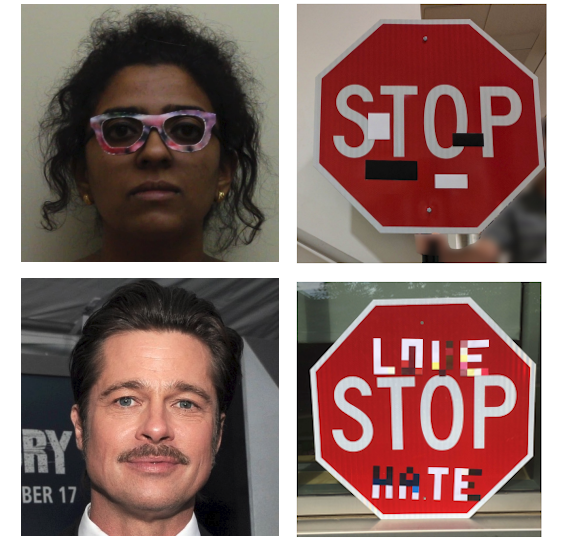
\includegraphics[width=0.3\textwidth]{threat_real.png}
    \caption{(links) Een bril die de perturbatie introduceert en leid tot de misclassificatie van de persoon die de bril draagt. (rechts) Stickers aangebracht op een stopbord die leiden tot misclassificatie van het bord.}
    \label{fig:realthreat}
\end{figure}

\subsection{Threat model}

Het generen van een adversarial example hangt af van de kennis die een aanvaller beschikt over het aan te vallen model, de intentie van de aanvaller en waartoe dat de aanvaller in staat is. Deze drie aspecten vormen het threat model en liggen aan de basis van het aanvallen en verdedigen van machine learning modellen. \\
\begin{itemize}
    \item \textbf{Beschikbare informatie over het model} \\ 
        De informatie die een aanvaller heeft over het model bepaald op welke manier hij/zij adversarial examples kan genereren. Zoals beschreven in \cite{Biggio_2013} kan de aanvaller beschikken over informatie over verschillende aspecten behorende het target model:
        \begin{itemize}
            \item De training data of een deel hiervan
            \item Hoe samples gerepresenteerd worden in de feature space van het model
            \item Het type van algoritme dat gebruikt wordt of de mogelijke architectuur
            \item Het volledige model: parameters van het model
            \item feedback van het model: is de aanvaller in staat het model te queryen om de bijhorende labels te verkrijgen
        \end{itemize}
        Afhankelijk van de graad van kennis kan de aanvaller adversarial examples genereren. Zo worden er in het geval van volledige kennis over het model gesproken over \textbf{white box} attacks en in het geval van geen informatie over \textbf{black box attacks}. Deze kunnen nog verder verdeelt worden in verband met de exacte kennis, zo is het mogelijk dat een black box model gequeryed kan worden om labels te verkrijgen of een white box model niet volledig gekend is maar enkel de parameters en architectuur. In de volgende sectie worden verschillende scenario's van kennis beschouwd en de aanvallen die hierbij aansluiten.
    \item \textbf{Wat zijn de mogelijkheden van de aanvaller}
        In de vorige sectie hebben we gesproken over de verschillende types van aanvallen: evasion attacks, posioning attacks en privacy attacks. Het is mogelijk dat de aanvaller de training data kan beïnvloeden wat kan leiden tot posioning attacks, evasion attacks zijn mogelijk indien de aanvaller het model kan gebruiken tijdens de test fase. \\ Indien de aanvaller een adversarial example genereert is het in veel gevallen wenselijk dat deze nog steeds gelijkaardig is aan de originele input, hierdoor is de noise die wordt toegepast gelimiteerd. Adversarial examples worden vervolgens gegenereerd gebaseerd op een $l_p$ gebonden norm. De meest gebruikte $l_p$ normen zijn de volgende:
        \begin{itemize}
            \item $l_0$ : Het aantal verschillende pixels tussen de originele input en het adversarial example.
            \item $l_2$ : Het kwadratisch verschil de originele input en het adversarial example.
            \item $l_{\infty}$: Het maximale verschil van pixel-waardes tussen de originele input en het advesarial examples.
        \end{itemize} 
        
        
        De gebruikte norm heeft een invloed op de adversarial examples die gegenereerd kunnen worden. De $l_\infty$ houdt enkel rekening met de maximaal veranderde pixel en niet het aantal veranderde pixels. De $l_0$ en $l_2$ normen limiteren het aantal pixels dat er verandert. 
        
        In praktijk wordt er vooral gebruikt gemaakt van de $l_\infty$ norm omdat de $l_0$ en vooral de $l_2$ zeer groot worden in het geval van willekeurige noise (niet specifieke noise zoals bij het genereren van adversarial examples) zonder een misclassificatie te veroorzaken. Vervolgens stelt de $l_2$ norm de aanvaller toe om de perturbaties te limiteren op een klein aantal pixels en deze tot extreme mate aan te kunnen passen waarbij dat er volledig witte of zwarte pixels kunnen worden geintroduceerd.
        
    \item \textbf{Doel van de aanvaller}
    
    
\end{itemize}

\section{Related work}

\bibliography{references.bib}
\end{multicols*}
\end{document}
